%!TEX root = TDT4265-Summary.tex
\section{Morphological image processing}
Morphology is image manipulation via set theory. It's pretty cool. Sort of like spatial filtering, but with nonlinear operations.

%%%%%%%%%%%%%%%%%%%%%%%%%%%%%%%%%%%%%%%%%%%%%%%%%%%%%%%%%%%%
\subsection{Preliminaries}
In morphology, images are represented as sets. Usually images are binary, and the set of an image is the set of 1-valued pixels, defined on $\mathbb{Z}^2$. An extension in $\mathbb{Z}^3$ to greyscale exists, and also to color and so on.

\subsubsection{Some set theory}
\begin{itemize}
    \item The absolute complement of a set $A$ is
    \begin{equation}
        A^c = \{ w | w \notin A \},
    \end{equation}
    which is all elements outside of $A$.
    \item The relative complement between two sets $A$ and $B$ is
    \begin{equation}
        A \setminus B = \{ w | w \in A, w \notin B \},
    \end{equation}
    which is all elements that are \emph{only} in $A$.
    \item The reflection (180 degree rotation) of a set is
    \begin{equation}
        \hat{B} = \{ w | w = -b \mbox{ for } b \in B \}.
    \end{equation}
    \item The translation of a set $A$ by a vector $z = (z_1, z_2)$ is
    \begin{equation}
        (B)_z = \{ c | c = b + z \mbox{ for } b \in B \}
    \end{equation}
\end{itemize}

\subsubsection{Structuring elements (SEs)}
An SE is a small subimage or subset that is used to find properties of the image. They are usually symmetric and with their center defined in the middle.

%%%%%%%%%%%%%%%%%%%%%%%%%%%%%%%%%%%%%%%%%%%%%%%%%%%%%%%%%%%%
\subsection{Erosion and dilation}

\subsubsection{Erosion}
The erosion of $A$ by $B$ is defined as
\begin{equation}
    A \erode B = \left\{ z | (B)_z \subseteq A \right\},
\end{equation}
which is the set of all points where $B$ is completely inside $A$. ($A$ is an image and $B$ is an SE.) The operation shrinks objects, and removes anything smaller/thinner than the SE, such as thin lines.

\subsubsection{Dilation}
The dilation of $A$ by $B$ is defined as
\begin{equation}
    A \dilate B = \left\{ z | (\hat{B})_z \cap A \neq \emptyset \right\}
\end{equation}
which is the set of all points where $\hat{B}$ (the reflection of $B$) overlaps with $A$ by at least one element. This operation grows objects, and can fill gaps and small holes.

\subsubsection{Duality}
Erosion and dilation are dual operations:
\begin{equation}
\begin{split}
    (A \erode  B)^c &= A^c \dilate \hat{B} \\
    (A \dilate B)^c &= A^c \erode  \hat{B} \\
\end{split}
\end{equation}
This is useful for symmetric SEs ($\hat{B} = B$), because then we can erode $A$ by instead dilating the background $A^c$.

%%%%%%%%%%%%%%%%%%%%%%%%%%%%%%%%%%%%%%%%%%%%%%%%%%%%%%%%%%%%
\subsection{Opening and closing}\label{ssec:open-close}
\emph{Opening} is defined as
\begin{subequations}
\begin{align}
    A \open B &= (A \erode B) \dilate B \\
              &= \bigcup \left\{ (B)_z | (B)_z \subseteq A \right\} \label{eq:opening-as-set}
\end{align}
\end{subequations}
It is analogous to the area defined by moving a ball (or other shape) along the inner boundary of a set, as in Figure \ref{fig:openclose}. Equation \eqref{eq:opening-as-set} shows that opening can be expressed as ``all translates of $B$ that fit inside $A$''. Used for e.g. removing thin connections between components and removing noise pixels.

\emph{Closing} is defined as
\begin{equation}
    A \close B = (A \dilate B) \erode B,
\end{equation}
which is analogous to the area defined by moving e.g. a ball along the outer boundary of a set, as in Figure \ref{fig:openclose}. Used for e.g. filling holes.

\begin{figure}[htbp]
    \centering
    \subfigure[Opening]{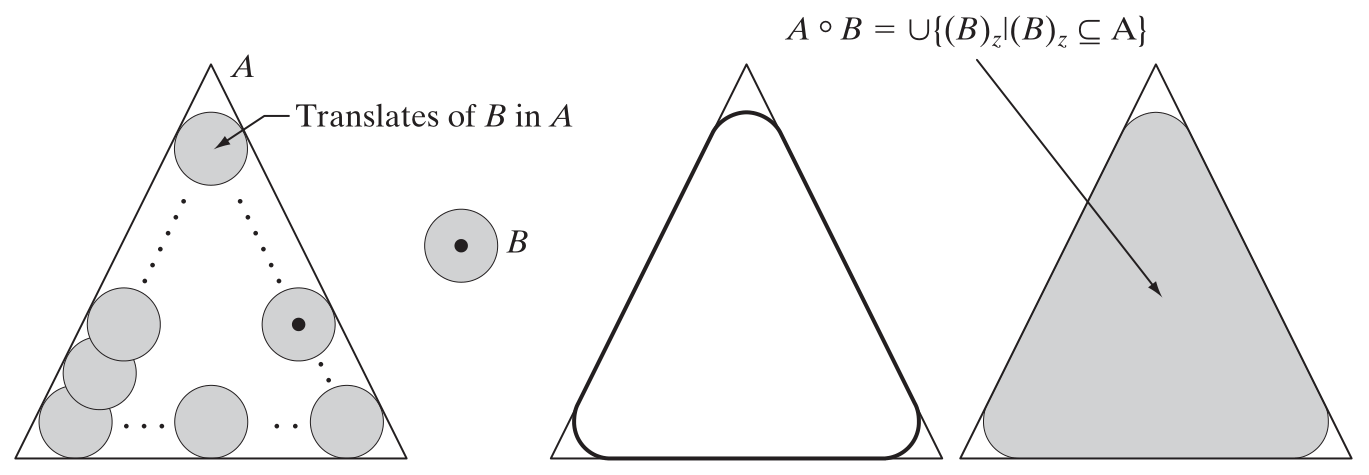
\includegraphics[width=.9\linewidth]{images/opening.png}} \\
    \subfigure[Closing]{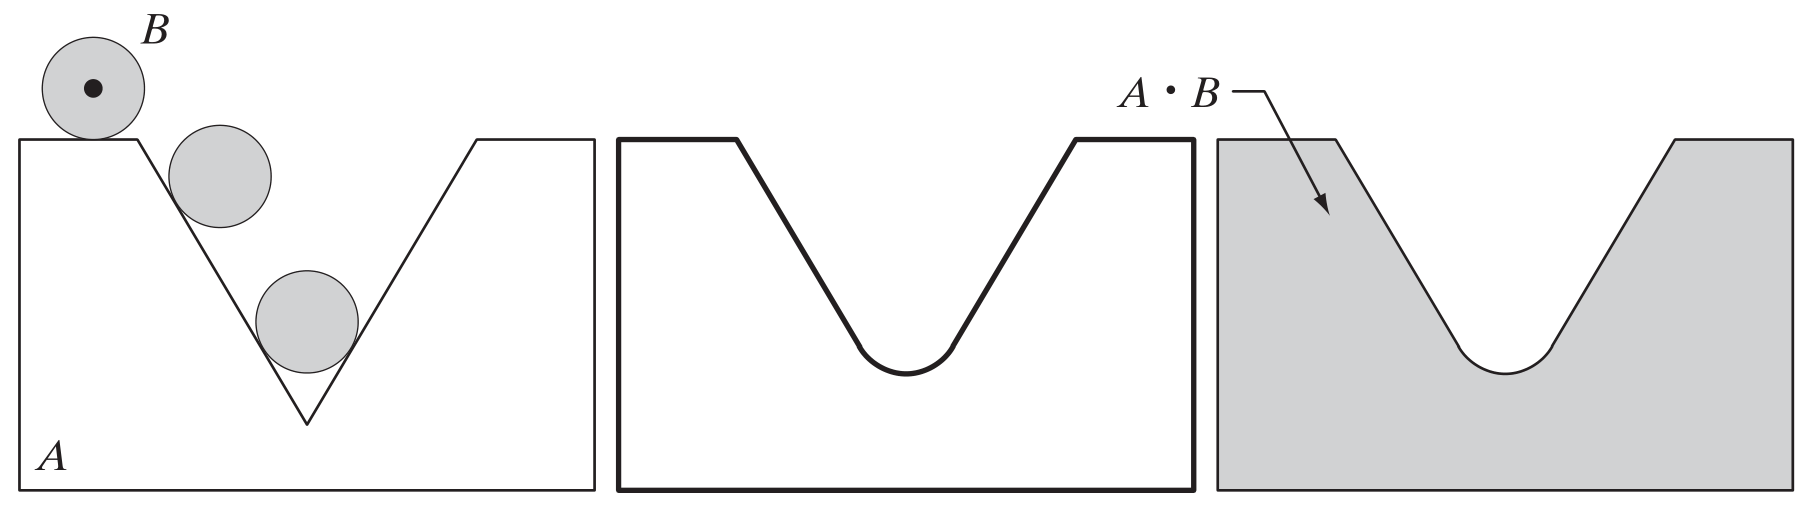
\includegraphics[width=.9\linewidth]{images/closing.png}}
    \caption{Analogies to the opening and closing operations}
    \label{fig:openclose}
\end{figure}

Note that both opening and closing are idempotent operations.

\paragraph{Combining opening and closing}
Opening followed by closing can remove noise, both specks of object pixels on the background and background pixels where there should be object. However, some connectivity may be lost.

%%%%%%%%%%%%%%%%%%%%%%%%%%%%%%%%%%%%%%%%%%%%%%%%%%%%%%%%%%%%
\subsection{The hit-or-miss transformation}
A basic tool for shape detection. Let $B = (B_1, B_2)$, $B_1$ be an object, and $B_2$ its background. Then the matches of $B$ in $A$ is
\begin{equation}
    A \match B = (A \erode B_1) \cap (A^c \erode B_2).
\end{equation}
The set $(A \erode B_1)$ are all locations where the object fits in, and $(A^c \erode B_2)$ are all locations where the background fits. Locations where both fit are locations of all shapes in $A$ that perfectly match $B$. We assume that each object we want to find is separate from the other objects, and therefore each has a complete local background at least one pixel wide.

%%%%%%%%%%%%%%%%%%%%%%%%%%%%%%%%%%%%%%%%%%%%%%%%%%%%%%%%%%%%
\subsection{Some basic morphological algorithms}
Now we can finally use this stuff.

\subsubsection{Boundary extraction}
Get the boundary by subracting the eroded image from the original.
\begin{equation}
    \beta(A) = A - (A \erode B)
\end{equation}
The erosion gives a ``smaller'' version of $A$, and subtracting that from the image leaves only the border.

\subsubsection{Hole filling}
Same principle as in Section \ref{sec:extract-connected} below.
\begin{equation}
    X_k = (X_{k-1} \dilate B) \cap A^c
\end{equation}
The seed pixel must be in a hole. It will grow until it fills the hole. Stop when no further change happens.

\subsubsection{Extraction of connected components}\label{sec:extract-connected}
Done by iteration:
\begin{equation}
    X_k = (X_{k-1} \dilate B) \cap A
\end{equation}
Choose a starting pixel (seed) $X_0$. Dilate $X_0$, but only keep the pixels that are in the original. Continue dilating and only keeping pixels present in $A$ until convergence.

\subsubsection{Convex hull}\label{sec:convex-hull}
A set is convex if any line segment between two points in the set lies fully within the set. The \emph{convex hull} $H$ of a set $S$ is the smallest convex set containing $S$. The difference $H - S$ is the \emph{convex decifiency} of $S$. It can be computed by iterating
\begin{equation}
    X_k^i = (X_{k-1} \match B^i) \cup A
    ,\quad i = 1,2,3,4
    ,\quad k = 1,2,\dots
\end{equation}
with $X_0^i = A$ and $B^i$ being as shown in Figure \ref{fig:convex-hull-SE}. For each SE, let $D^i = X_k^i$ when its iteration converges. Then the convex hull is
\begin{equation}
    C(A) = \bigcup_{i=4}^{4} D^i
\end{equation}

\begin{figure}[htbp]
    \centering
    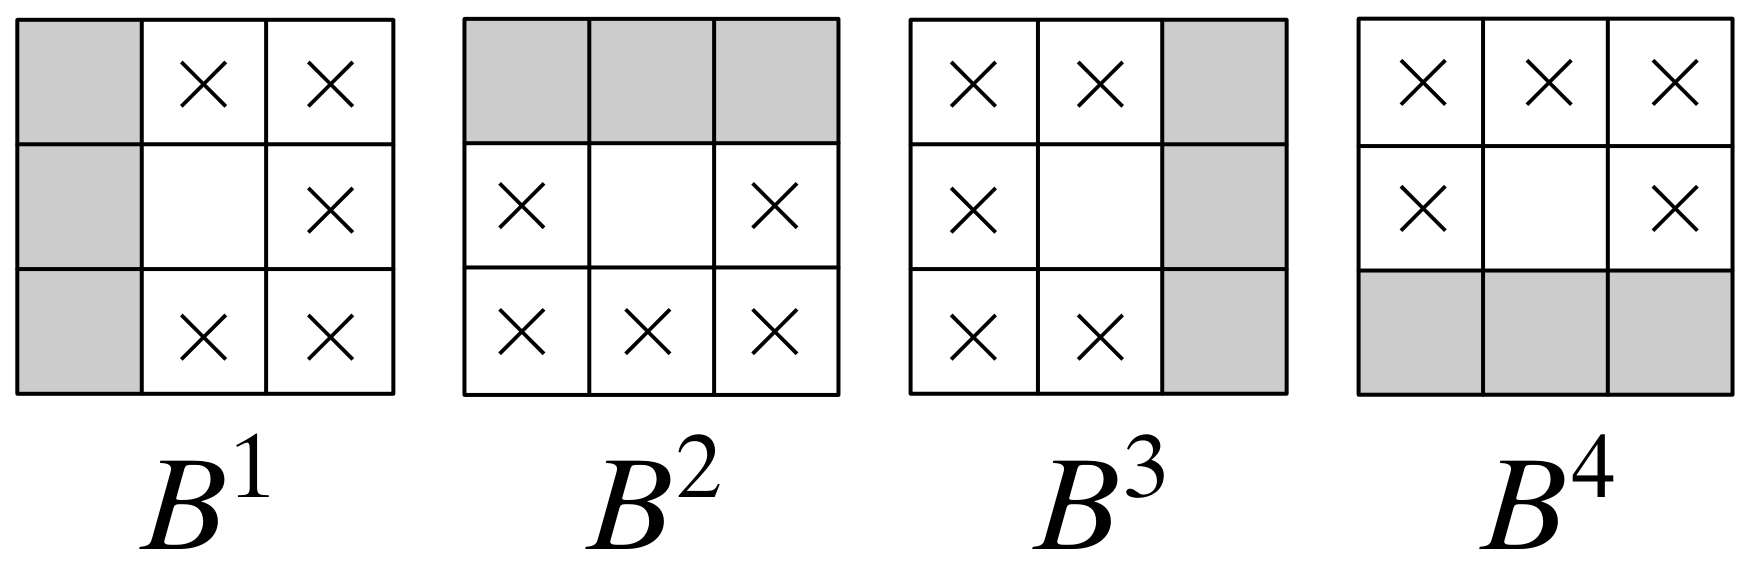
\includegraphics[width=.5\linewidth]{images/SE-for-convex-hull.png}
    \caption{SEs for convex hull extraction}
    \label{fig:convex-hull-SE}
\end{figure}

\subsubsection{Thinning}\label{sec:thinning}
Used e.g. for skeletonization and to thin edge detector output. It is defined in terms of the hit-or-miss transformation as
\begin{equation}
    A \thin B = A \cap (A \match B)^c
\end{equation}
with a sequence of SEs
\begin{equation}
    \{ B \} = \{ B^1, \dots, B^n \}
\end{equation}
where $B^i$ is a rotated $B^{i-1}$. Then just keep applying hit-or-miss with $B$ repeatedly, until continuing has no effect.

One pass of thinning is written as
\begin{equation}
    A \thin \{ B \} = ((\dots ((A \thin B^1) \thin B^2) \dots ) \thin B^n)
\end{equation}

\subsubsection{Thickening}
Thickening is the dual of thinning:
\begin{equation}
    A \thick B = A \cup (A \match B)
\end{equation}

\subsubsection{Skeletons}
The skeleton is
\begin{equation}
    S(A) = \bigcup_{k=0}^{K} (A \erode kB) - (A \erode kB) \open B
\end{equation}
where $B$ is an SE and $(A \erode kB)$ indicates $k$ successive erosions of $A$. $K$ is the number of erosions possible before resulting in the empty set.

\subsubsection{Pruning}
Skeletons often have unwanted ``spurs''. Assuming the spurs are sufficiently small, pruning can remove them. We perform thinning with SEs designed to only detect end points.
\begin{equation}
    X_1 = A \thin \{B\}
\end{equation}
The SEs used are shown in Figure \ref{fig:se-for-pruning}.

\begin{figure}[htbp]
    \centering
    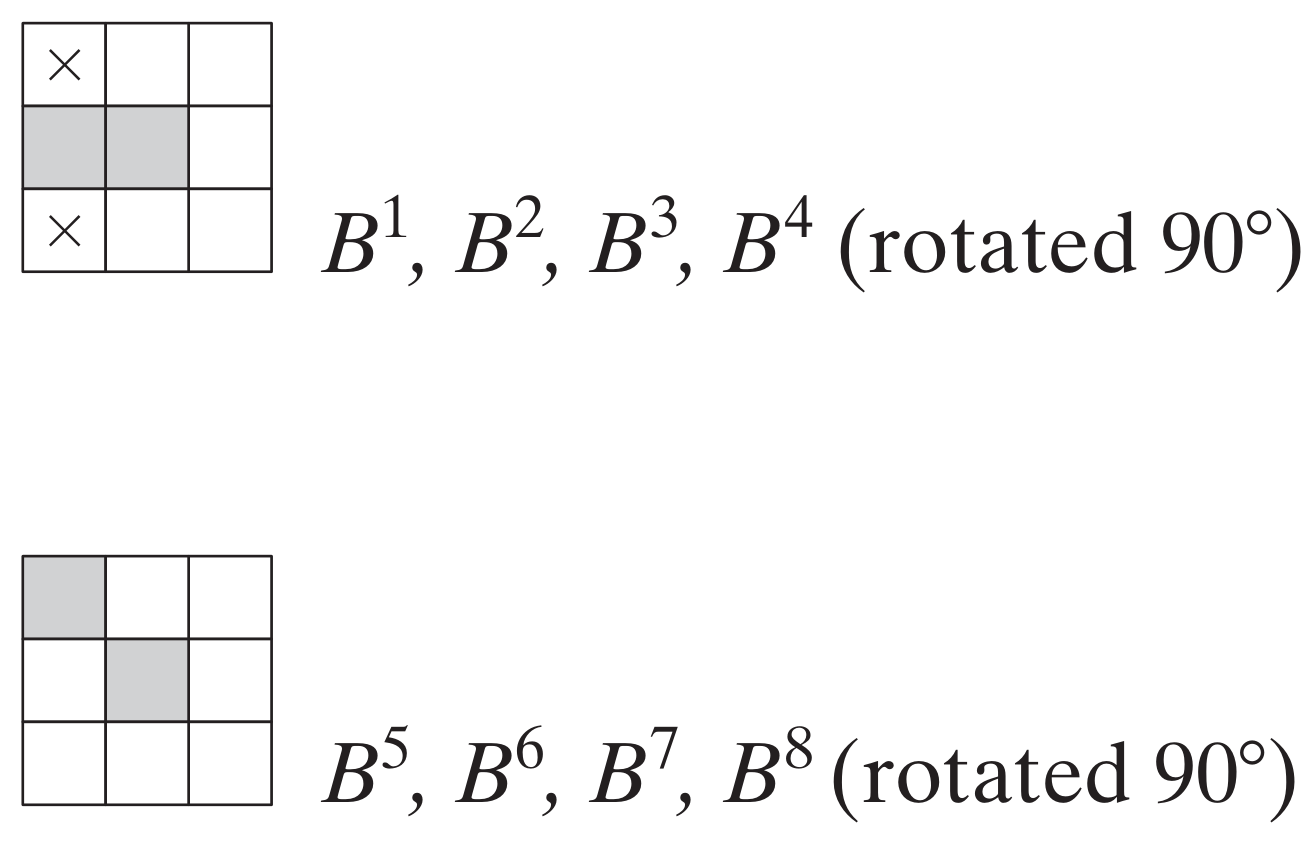
\includegraphics[width=0.5\linewidth]{images/SE-for-pruning.PNG}
    \caption{SEs for pruning}
    \label{fig:se-for-pruning}
\end{figure}

\subsubsection{Morphological reconstruction}
Uses two images, a marker $F$ with starting points, and a mask $G$ that constrains the transformation.

\paragraph{Geodesic dilation}
Geodesic dilation is the intersection of the mask and the dilated marker. One pass is
\begin{equation}\label{eq:geo-dilation}
    D_G^{(1)}(F) = (F \dilate B) \cap G.
\end{equation}
Several passes, denoted $D_G^{(n)}$, is just repeating the operation $n$ times.

\paragraph{Geodesic erosion}
Geodesic erosion is the union of the mask and the eroded marker. One pass is
\begin{equation}\label{eq:geo-erosion}
    E_G^{(1)}(F) = (F \erode B) \cup G.
\end{equation}

\paragraph{Morphological reconstruction by dilation}
Reconstruction by dilation is just repeating \eqref{eq:geo-dilation} until more passes have to effect:
\begin{equation}
    R_G^D(F) = D_G^{(k)}(F)
\end{equation}

\paragraph{Morphological reconstruction by erosion}
Same as by dilation, but using erosion:
\begin{equation}
    R_G^E(F) = E_G^{(k)}(F)
\end{equation}

\paragraph{Opening by reconstruction}
With normal opening (Section \ref{ssec:open-close}), erosion removes small things and dilation restores the original size/shape. Opening by reconstruction restores the precise original shape, and is done as reconstruction by dilation of $F$, from the erosion of size $n$ of $F$:
\begin{equation}
    O_R^{(n)}(F) = R_F^D \left[ (F \erode nB) \right]
\end{equation}
where $(F \erode nb)$ indicates $n$ erosions.

The SE for erosion $B$ determines the shapes we want to identify. The erosion itself leaves us with markers for all matching objects (because they are not removed by the erosion). Then, the image $F$ is used as a mask, and reconstruction is done by dilating the markers, subject to the mask. That way, all objects marked will be completely filled, and the result is removing all unmarked objects.

\paragraph{Filling holes}
With morphological reconstruction we can fill holes automatically, without knowing where they are. Create a marker image $F$ of zeros, except for the border, where it is $1 - I$. Then
\begin{equation}
    H = \left[ R_{I^c}^D(F) \right]^c
\end{equation}
is $I$ with all holes filled.

\paragraph{Border clearing}
Morphological reconstruction can also be used to remove objects connected to the borders of an image. Create a marker image $F$ that is equal to the input image $I$ at the border, and 0 elsewhere. We can extract all border-touching objects by the morphological reconstruction $R_I^D(F)$, and subtract it from the original to get an image without border objects $X$:
\begin{equation}
    X = I - R_I^D(F)
\end{equation}

\subsubsection{Summary}
We have now defined the following morphological operations:
\begin{itemize}
    \item Basic set operations:
    \begin{itemize}
        \item Translation
        \item Reflection
        \item Complement
        \item Difference
    \end{itemize}
    \item Basic morphological operations:
    \begin{itemize}
        \item Erosion
        \item Dilation
        \item Opening
        \item Closing
    \end{itemize}
    \item Complex morphological operations:
    \begin{itemize}
        \item Hit-or-miss transform
        \item Boundary extraction
        \item Hole filling
        \item Connected components
        \item Convex hull
        \item Thinning
        \item Thickening
        \item Skeletons
        \item Pruning
    \end{itemize}
    \item Morphological reconstruction operations:
    \begin{itemize}
        \item Geodesic dilation
        \item Geodesic erosion
        \item Morphological reconstruction by dilation
        \item Morphological reconstruction by erosion
        \item Opening by reconstruction
        \item Closing by reconstruction
        \item Hole filling
        \item Border clearing
    \end{itemize}
\end{itemize}

%%%%%%%%%%%%%%%%%%%%%%%%%%%%%%%%%%%%%%%%%%%%%%%%%%%%%%%%%%%%
\subsection{Grey-scale morphology}
We can dilate, erode, open, and close grey-scale images too! Now we use images $f(x,y)$ and SEs $b(x,y)$. The SEs can now be either flat (uniform) or nonflat. We stick to flat SEs for simplicity.

\subsubsection{Erosion and dilation}
Erosion of $f$ by a flat SE $b$ is the minimum value of the image in the region covered by the SE:
\begin{equation}
    \left[ f \erode b \right](x,y) = \min_{(s,t) \in b} \left\{ f(x+s, y+t) \right\}.
\end{equation}
Dilation is similarly
\begin{equation}
    \left[ f \dilate b \right](x,y) = \max_{(s,t) \in b}  \left\{ f(x-s, y-t) \right\},
\end{equation}
which uses  $\hat{b} = b(-x,-y)$.

\subsubsection{Opening and closing}\label{sssec:greyscale-open-close}
This is mathematically just as before:
\begin{subequations}
\begin{align}
    f \open b = (f \erode b) \dilate b \\
    f \close b = (f \dilate b) \erode b
\end{align}
\end{subequations}

Looking at the image as a topographic surface, opening is pushing the SE up from below, clipping all peaks where it doesn't fit, and closing is pushing the SE down from above, clipping all valleys where it doesn't fit. See Figure \ref{fig:greyscale-opening-closing}. This means that opening removes small, bright details, and closing removes small, dark details.

\begin{figure}[htbp]
    \centering
    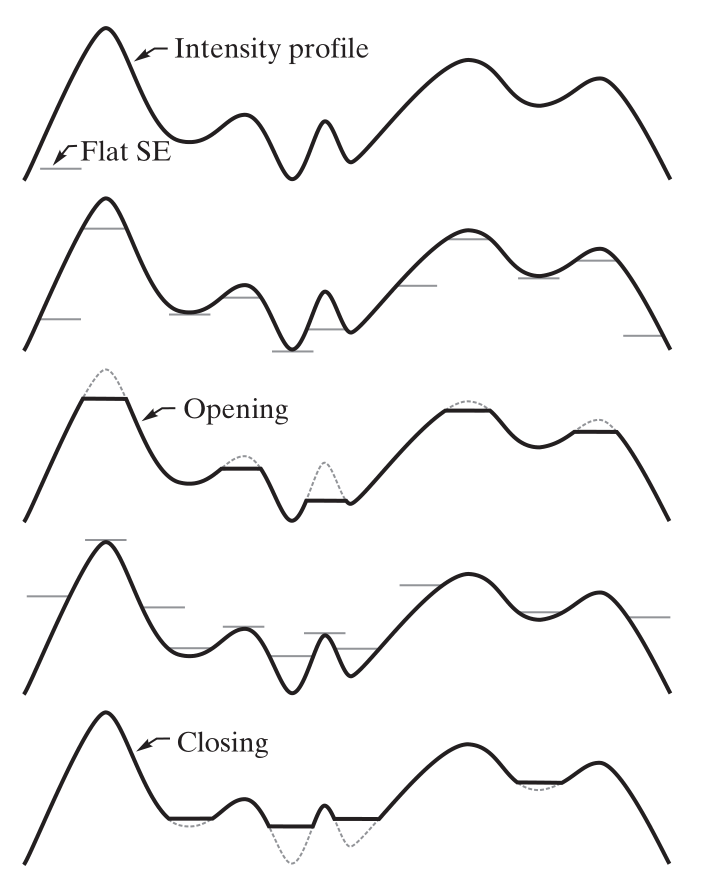
\includegraphics[width=0.8\linewidth]{images/greyscale-opening-closing}
    \caption{Analogy to opening and closing greyscale images}
    \label{fig:greyscale-opening-closing}
\end{figure}

\subsubsection{Some basic greyscale morphological algorithms}

\paragraph{Smoothing}
The ``small bright/dark details'' mentioned in Section \ref{sssec:greyscale-open-close} might be noise. This means we can remove this type of noise by opening and then closing. The size of the SE then sets a threshold for what is image and what is noise.

\paragraph{Morphological gradient}
The morphological gradient is
\begin{equation}
    g = (f \dilate b) - (f \erode b).
\end{equation}
The dilation thickens objects in the image, and the erosion shrinks them. Differencing these emphasises edges and removes homogenous areas, which gives a gradientlike effect.

\paragraph{Top-hat and bottom-hat transformations}\label{par:top-hat}
Subtracting the opening of an image from the image itself defined the top-hat transformation
\begin{equation}
    T\sub{hat}(f) = f - (f \open b).
\end{equation}
The bottom-hat transformation is defined similarly:
\begin{equation}
    B\sub{hat}(f) = (f \close b) - f
\end{equation}

Top-hat can isolate light objects on a dark background, and bottom-hat does the opposite. This is a type of segmentation, and works well even with uneven lightning.

Opening with an SE that is too large to fit in the objects you want to segment will remove all such objects and leave only an approximation of the background, including any uneven lightning. If you subtract the approximate background from the original, the unevenness will be reduced, and now thresholding methods can be used with success.

\paragraph{Granulometry}
(Assuming light objects on a dark background.) Open the image with gradually larger SEs, and compute the sum of pixel values. As the SEs grow larger than the objects, they disappear, and the pixel sum decreases. Plotting pixel sum against SE size indicates by peaks in the plot the predominant sizes of objects in the image. This can be used to simply get the size distribution of objects, but also to identify defect objects (sizewise).

\paragraph{Textural segmentation}
(Assuming light objects on a dark background.) Textural segmentation is to divide an image into regions based on their texture contents. If you have an image with some coarse and some fine texture, you can close it with an SE large enough to remove the fine objects. Then open it with an SE large enough to fill the gaps between the coarse objects. Now coarse areas are dark, and fine areas are bright, and the boundary can be extracted by e.g. a morph. gradient.

\subsubsection{Greyscale morphological reconstruction}
Let $f$ be the marker, and $g$ be the mask. The basic operations are similar to their black-and-white counterparts.
\begin{itemize}
    \item Geodesic dilation:
    \begin{equation}
        D_g^{(1)}(f) = (f \dilate b) \wedge g
    \end{equation}
    \item Geodesic erosion:
    \begin{equation}
        E_g^{(1)}(f) = (f \erode b) \vee g
    \end{equation}
    \item Reconstruction by dilation:
    \begin{equation}
        R_g^D(f) = D_g^{(k)}(f)
    \end{equation}
    \item Reconstruction by erosion:
    \begin{equation}
        R_g^E(f) = E_g^{(k)}(f)
    \end{equation}
    \item Opening by reconstruction:
    \begin{equation}
        O_R^{(n)}(f) = R_f^D \left[ (f \erode nb) \right]
    \end{equation}
    \item Closing by reconstruction:
    \begin{equation}
        C_R^{(n)}(f) = R_f^E \left[ (f \dilate nb) \right]
    \end{equation}
\end{itemize}

\paragraph{Top-hat by reconstruction}
This method consists of subtracting an image's opening by reconstruction from the image.
